\chapter{State Estimation}
\label{ch:st_est}
The state estimation is the principle of estimating the internal state(s) of the system from the measurement of input(s) and output(s) of the system. The knowledge of the internal state of the system will make the system easier to control. Figure \ref{fig:observer} shows the setup of state estimator in state feedback control loop.
\begin{figure}[h]
%  \centering
%  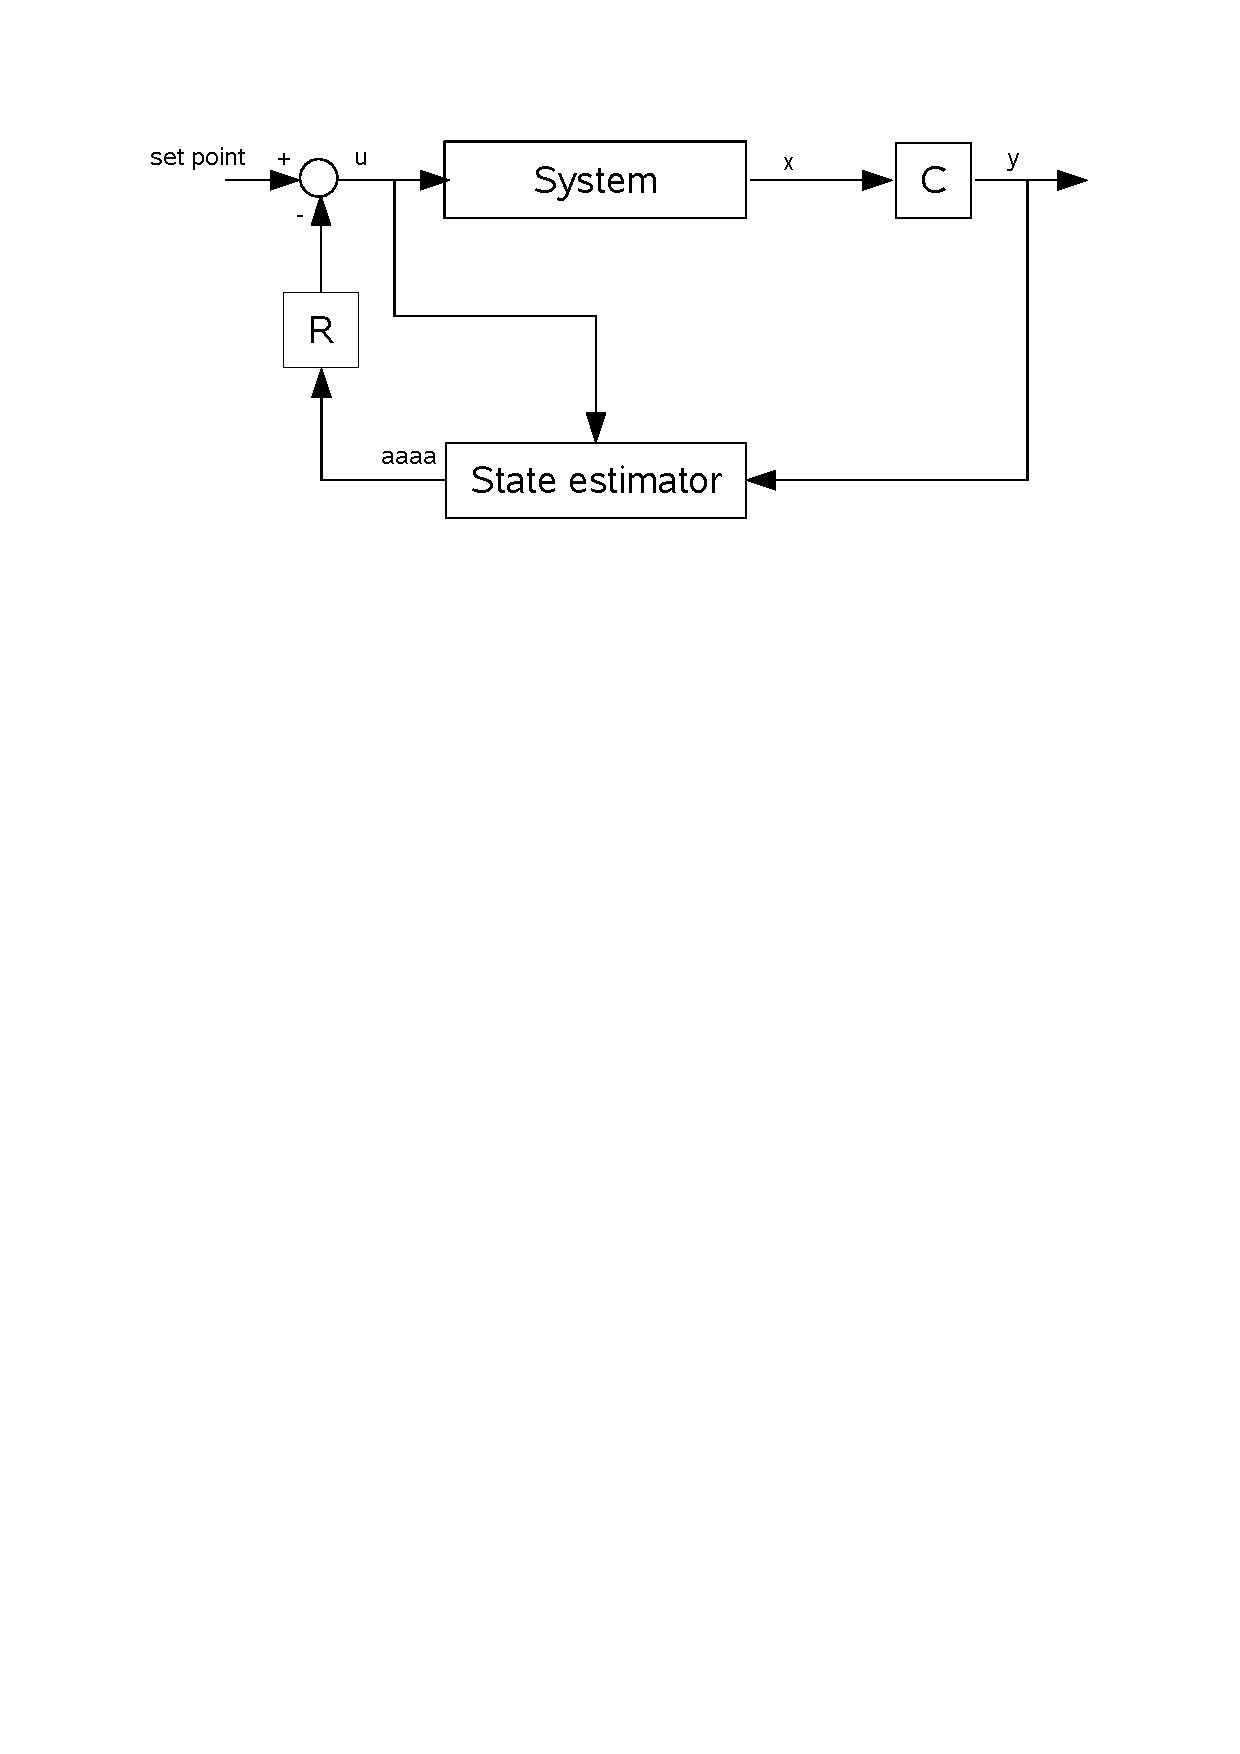
\includegraphics[trim = 10mm 200mm 20mm 20mm, clip,scale=0.80]{Bilder/system_observer.pdf}
\tikzstyle{block} = [draw, fill=blue!20, rectangle, 
    minimum height=3em, minimum width=6em]
\tikzstyle{sum} = [draw, fill=blue!20, circle, node distance=1cm]
\tikzstyle{input} = [coordinate]
\tikzstyle{output} = [coordinate]
\tikzstyle{pinstyle} = [pin edge={to-,thin,black}]
\def\blockdist{2.3}
% The block diagram code is probably more verbose than necessary
\begin{tikzpicture}[auto, node distance=4cm,>=latex']
    % We start by placing the blocks
    \node [input, name=input] {};
    \node [sum, right of=input] (sum) {};
    \node [block, right of=sum] (controller) {Controller};
    \node [block, right of=controller, pin={[pinstyle]above:Disturbances},
            node distance=5cm] (system) {System};
    % We draw an edge between the controller and system block to 
    % calculate the coordinate u. We need it to place the measurement block. 
    \draw [->] (controller) -- node[name=u] {$u$} (system);
    \node [output, right of=system] (output) {};
    \node [block, below of= controller] (measurements) {Estimator};

    % Once the nodes are placed, connecting them is easy. 
    \draw [draw,->] (input) -- node {$r$} (sum);
    \draw [->] (sum) -- node {$e$} (controller);
    \draw [->] (system) -- node [name=y] {$y$}(output);
    \draw [->] (y) |- (measurements.base east);
    \draw [->] (u) |- (measurements.10);
    \draw [->] (measurements) -| node[pos=0.99] {$-$} 
        node [near end] {$\hat{x}$} (sum);
\end{tikzpicture}
    \caption{State feedback controller with state estimator}
      \label{fig:observer}
\end{figure}

The state space equations of a nonlinear system is
\begin{equation}
\begin{split}
\label{eqn:nl_sys}
\dot{x}(t) &= f(x(t),u(t)) , x(t=0) = x_0 \\
y(t) &= g(x(t),u(t)),
\end{split}
\end{equation}

where $t$ is a scalar representing time, $x(t)$ represents the state vector, $u(t)$ represents the input vector and $y(t)$ represents the output vector of the system. The state $x(t)$,input $u(t)$ and output $y(t)$ depends on time $t$. The variable $x_0$ represents the vector of initial states $x(t=0)$ of the system. 
The state space equations of the state estimator is 
\begin{equation}
\begin{split}
\label{eqn:est_sys}
\dot{\hat{x}}(t) &= f(\hat{x}(t),u(t)) + K(y(t)-\hat{y}(t)) , \hat{x}(t=0) = \hat{x}_0  \\
\hat{y}(t) &= g(\hat{x}(t),u(t)),
\end{split}
\end{equation}
where $\hat{x}(t)$ \footnote{ The estimated states are represented by hat symbol at the top, inorder to differentiate them from the true states of the system. For example $\hat x_k$ represents the estimated states} is the state vector of estimator and $K$ is the estimator gain matrix.  A state estimator should satisfy the following properties \citep{gre01}:
\begin{itemize}
\item \textbf{Simulation property:} When the estimator and the system to be observed have same initial condition $x_0 = \hat{x}_0$, then it holds that $x(t) = \hat{x}(t) \forall t > 0 $
\item \textbf{Convergence property:} If $x_0 \neq \hat{x}_0$, then $x(t) - \hat{x}(t)$ tends to zero as $ t \rightarrow \infty $.
\end{itemize}

There are different methods for computing the estimator gain matrix $K$ in Equation \ref{eqn:est_sys}. The Luenberger observer has a deterministic way of computing the gain for linear systems. The sliding mode observer and Kalman filter determines the gain matrix by minimizing the error between the estimates $\hat{x}$ and actual states $x$ \citep{kha02}.